\begin{figure}
  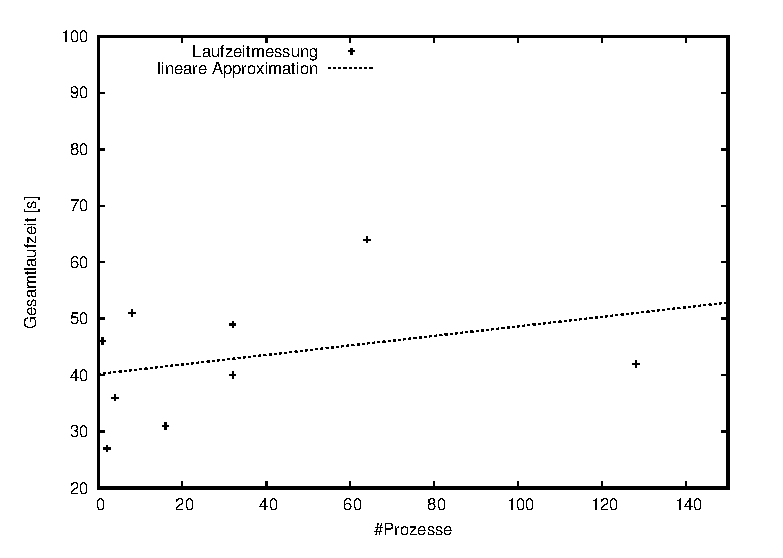
\includegraphics{img/grav_X20_lin.eps}
  \caption{Dieses Diagramm zeigt den Anstieg der Laufzeit in Abhängigkeit zur Anzahl Prozesse.}
  \label{fig:x20}
\end{figure}

\begin{table}[]
  \begin{tabular}{|c|c|}
    \hline
    \#Prozesse & Laufzeit [s] \\
    \hline
    1 & 46,54 \\
    2 & 27,73 \\
    4 & 36,94 \\
    8 & 51,94 \\
    16 & 31,29 \\
    32\footnote{Die 32 Prozesse befanden sich auf einem Knoten des Clustersystems.} & 49,42 \\
    32\footnote{Die 32 Prozesse verteilten sich zu je 16 auf zwei Knoten des Clustersystems.} & 40,82 \\
    64 & 64,96 \\
    128 & 42,27 \\
    \hline
  \end{tabular}
  \caption{Tabelle der gemessenen Laufzeitdaten in Abhängigkeit zur Anzahl Prozesse.}
  \label{tab:x20}
\end{table}

